\documentclass[compress,handout,10pt]{beamer}

\newlength{\wideitemsep}
\setlength{\wideitemsep}{\itemsep}
\addtolength{\wideitemsep}{100pt}
\let\olditem\item
\renewcommand{\item}{\setlength{\itemsep}{0.5\baselineskip}\olditem}

\usetheme{Singapore}
\usecolortheme{lily}
\usefonttheme[onlymath]{serif}

\usepackage{float}
\floatstyle{boxed}
\usepackage{colortbl}
\usepackage{mathpazo}
\usepackage{graphicx}
\usepackage{movie15}
\usepackage{bm}
\usepackage{verbatim}
\usepackage{comment}
\usepackage{caption}
\usepackage{subcaption}
\captionsetup[subfigure]{labelformat=empty}
\captionsetup[figure]{labelformat=empty}

\newcommand{\mygreen}{\color{green!50!black}}
\newcommand{\myblue}{\color{blue}}
\newcommand{\myred}{\color{red}}
\newcommand{\mycolor}{\color{red}{c}\color{blue}{o}\color{green}{l}\color{orange}{o}\color{cyan}{r}}
\newcommand{\mysize}{\scriptsize{s}\small{i}\normalsize{z}\Large{e}}
\newcommand{\myshape}{\textcircled{s}\textit{h}\texttt{a}\textsf{p}\textsc{e}}

\xdefinecolor{titlecolor}{rgb}{.855,.647,.125}
\setbeamercolor{frametitle}{fg=titlecolor}
\setbeamerfont{frametitle}{series=\bfseries}
\setbeamercolor{normal text in math text}{parent=math text}

\setbeamertemplate{navigation symbols}{} %gets rid of navigation symbols
\setbeamertemplate{footline}[frame number]
\beamertemplateshadingbackground{blue!5}{yellow!10}

\title{{\color{blue} \LARGE Portfolio Analysis and Suggestions for Jabre Capital\newline} }
\subtitle{{\color{red} \large Sponsored by Jabre Capital} }

\author{ 
%    \vspace{5pt}
    {\bf{Presenter:}} \\ 
T.~Luo \\ 
    \vspace{5pt}
} 
\institute{JHU AMS 2012 FALL}

\date{\mygreen Last Complied on \today} 

\begin{document}

\begin{frame}[plain]
    \titlepage
\end{frame}

\begin{frame}
    \frametitle{Outline}
    \tableofcontents
\end{frame}

\section{Background}

\begin{frame}
    \frametitle{Jabre Captial's Basic Information}
    Jabre Capital is an alternatve asset management platform founded in 2006. It provides sevices and products including:
    \vspace{7pt}
             \begin{enumerate}
                 \item Cayman-based collective investment schemes
                 \item UCITS IV regulated strategies 
                 \item Individually managed accounts
		 \end{enumerate}
\color{red}Jabre Capital is a diversified fund, which contains a wide array of securities to reduce the amount of risk in the fund.
\end{frame}
     
\section{Problem Statement}
\begin{frame}
    \frametitle{Jabre Capital's Changllenges}
The comparasion below clearly illustrates the challenge Jabre Capital faces:
\vspace{7pt}    
\begin{enumerate}
        \item As of December 31th 2010, Jabre Capital had portfolio value of \$4,133,365,000
	\item A year later, the portfolio value was only \$793,966,000
     \end{enumerate}
\color{red}    In one year, the hedge fund's value was down by around 80\%, which made it among the 10 worst hedge funds 2011.    
\end{frame}


\begin{frame}
    \frametitle{Manager's Puzzle}
Mr. Philippee Jabre, the fund manager, has the following puzzles:
\vspace{7pt}    
\begin{enumerate}
 \item  He had difficulties in finding support and resistance lines for call and put of a stock,
\item  Mr. Jabre did not have the right recipe for reducing risk and increasing diversification.   
\end{enumerate} 
\color{red} in 2012 Q2, the return of his S\&P's pick was -6.5\%, compared to total market gain 0.1\%. 
\begin{figure}[h]
    \begin{center}
        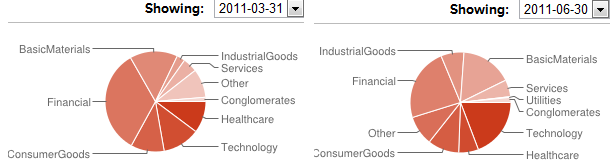
\includegraphics[width=\textwidth]{images/1.png}
    \end{center}
    \caption{Piechart of Stock Selection}
    \label{fig:Piechart}
\end{figure}  
\end{frame}

\begin{frame}
    \frametitle{Analysis of Manager's Puzzle}
Support and resistance represent key junctures where the forces of supply and demand meet.
\begin{itemize}
\item Support is the price level at which demand is thought to be strong enough to prevent the price from declining further, 
\item Resistance is the price level at which selling is thought to be strong enough to prevent the price from rising further.
\end{itemize}
If we can find lines where the price won't go above or below, they are support and resistance lines.
\begin{figure}[h]
    \begin{center}
        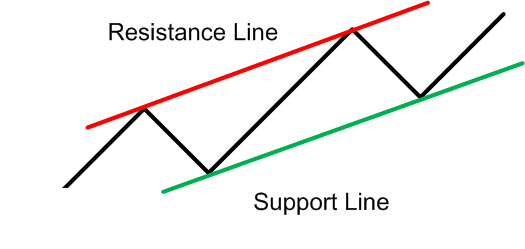
\includegraphics[width=2.5in]{images/2.png}
    \end{center}
    \caption{Support and Resistance Line}
    \label{fig:SRL}
\end{figure}  
\end{frame}

\begin{frame}
    \frametitle{Analysis of Manager's Puzzle}
The variance of return plot reflects how risky a stock is.\\
\begin{figure}[h]
    \begin{center}
        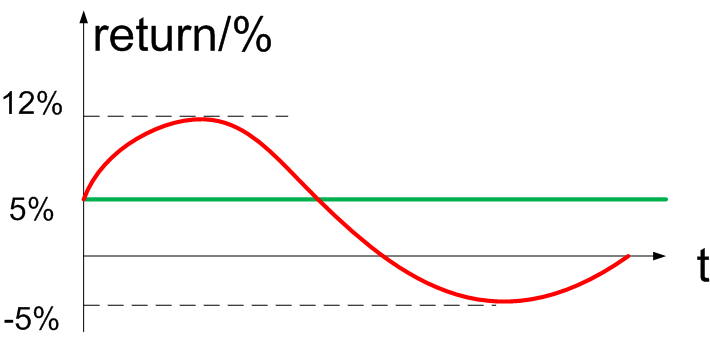
\includegraphics[width=2.5in]{images/6.png}
    \end{center}
    \caption{Return-time plots}
    \label{fig:RP}
\end{figure}
In financial market, risk usually cosists of two parts:
\vspace{7pt}    
\begin{itemize}
 \item  Systematic risk (undiversified risk): risk inherent to the entire market or entire market segment and  cannot be avoided through diversification.
\item  Unsystematic risk (diversified risk): Company or industry specific risk that is inherent in each investment. The amount of unsystematic risk can be reduced through appropriate diversification. 
\end{itemize} 
\end{frame}

\begin{frame}
\frametitle{Analysis of Manager's Puzzle}
In our model, the independent and dependent variables are as follows:
\begin{itemize}
\item Exogenous variable: systematic part of return variance
\item Endogenous variable: unsystematic part of return variance, the overal return variance
\end{itemize}

The challenges are:
\begin{itemize}
\item Systematic risk and unsystematic risk are mixed with each other. 
\item When the dimension of the data set increases, it becomes even harder to tell whether the diversification decreases the unsystematic risk of a specific portfolio.
\end{itemize}
\end{frame}

\begin{frame}
\frametitle{Analysis of Manager's Puzzle}
\begin{figure}[h]
\begin{center}
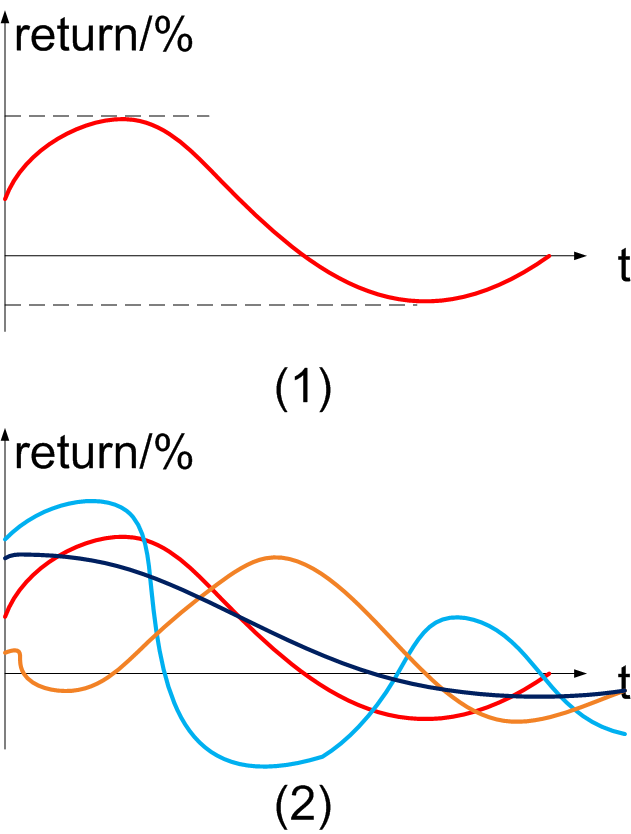
\includegraphics[width=2in]{images/7.png}
\end{center}
\caption{Comparasion of two portfolios}
\label{fig:ctp}
\end{figure}
\end{frame}

\begin{frame}
    \frametitle{Our Task}
Our task is to see:
\begin{enumerate}
\item Develop a software which will detect the support and resistance lines automatically.
 \item  Decide the large number of stock holdings (the number was more than 150 in Q1 2011)truly reduce the unsystematic risk or not.
\item  If the large stock holdings don't help improve the diversification, we will further our work to eliminate unnecessary stocks for Jabre Capital.
\end{enumerate}   
\end{frame}


\section{Approach of Task 1}
\begin{frame}
\frametitle{Algorithm Applied}
My approach for task 1 is as follows:
\begin{itemize}
\item Find points where the  derivative is about to change signal,
\item Find the maximum and minimum point among these points,
\item Among all the green points, draw a line which conects minimum point and another point with the smallest absolute value of slope rate,
\item Among all the red points, draw a line which conects minimum point and another point with the smallest absolute value of slope rate.
\end{itemize}
\begin{figure}[h]
    \begin{center}
        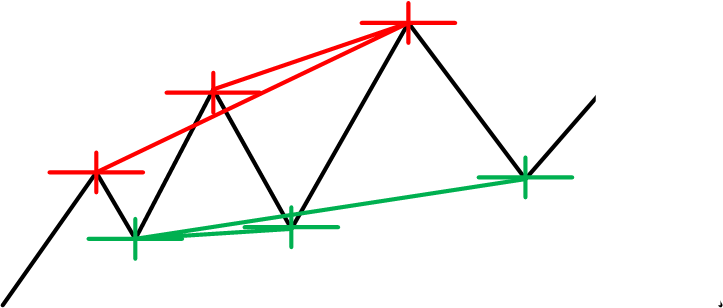
\includegraphics[width=\textwidth]{images/5.png}
    \end{center}
    \caption{Explanation of resistance and support lines}
    \label{fig:ers}
\end{figure}
\end{frame}

\section{Approach of Task 2 and 3}
\begin{frame}
    \frametitle{Introduction of Principal Component Analysis(PCA)}
Principal component analysis (PCA) is:\\
A mathematical procedure that converts a set of observations of possibly correlated variables into a set of values of linearly uncorrelated eigenvectors. 

Here is an example of PCA analysis:
	\begin{enumerate}
	\item Get some data and subtract the mean
	\item Calculate the covariance matrix 
	\item Calculate the eigenvectors and eignevalues of the covariance matrix
	\item Choose components, form a feature vector, and approximately predict data from the data set
	\end{enumerate}
It is a powerful method to find patterns in data of high dimension, and compress data to low dimension without losing much information.
\end{frame}

\begin{frame}
    \frametitle{Problem Solving based on PCA}
In our approach, we will use the return performance of a stock rather than price peformance, as the thing we are interested in is changes in the stock price rather than absolute stock prices.

Thus, to help Jabre Capital with its challenges, our approach will be divided into following steps:
\begin{enumerate}
\item Get historical prices of stocks ever on Jabre Capital's list in 2011, and develop historical return ratios accordingly,
\item Divide stocks accroding to industries they are in, and list important macro econimic factors(such as matrial prices) to a specific industry,
\item Gather historical data of the macro econimic factors, and decide whether these factors are favorable to stock performance or not,
\end{enumerate}
\end{frame}

\begin{frame}
    \frametitle{Problem Solving based on PCA}
\begin{itemize}
\item If macro econimc fators are favorable or neutral to a certain industry, apply Principal Component Analysis to find whether there is a specific return pattern in the industry,
	\begin{itemize}
	\item If there is a certain pattern, elect one stock with highest average return ratio and minimized risk to represent a specific industry,
	\item If there is no such pattern, divide stocks in the same industry into subcatogries to find whether there is a certain pattern or not, until the number of stocks in this industry decreases by 80\% which corresponds to the portfolio value loss.
	\end{itemize}
\item If macro ecnomic factors are not favorable to a certain industry, decide whether to exit this industry or not, by referring to authorized third party opnions about the factor's future trends.
\end{itemize} 

\end{frame}

\section{Deliverables}
\begin{frame}
    \frametitle{From Team to Sponsor}
The following outputs are expected from this project:
\begin{itemize}
    \item Software of finding support and resistance line,
    \item Return of Investment charts and data of all the stocks Jabre Capital invested in 2011,
    \item Principal component analysis of all the stocks, stocks in each industry, stocks in each subcategory,
    \item Suggestions about a narrowed portfolio list,
    \item R package with a complete set of documentations along with some test codes that can be used to reproduce simulation results,
    \item Technical report and presentations summarizing the work. 
\end{itemize}

\end{frame}

\begin{frame}
    \frametitle{From Sponsor to Team}
In order for our project to be of successful one, we will need:
\begin{itemize}
    \item Provide lists of stocks Jabre Capital held in 2011, and access to all the price charts and data of these stocks before Oct 26,2012
     \item Timely responses to inquiries, 
    \item Symposium attendance travel expenses.
\end{itemize}


\end{frame}

\section{Conclusion}
\begin{frame}
    \frametitle{Evaluation of Task 1}
Based on algorithm mentioned, I have developed software for drawing support and resistance lines. 
Using a sample data, I get the pictures as follows:
\begin{figure}[h]
    \begin{center}
        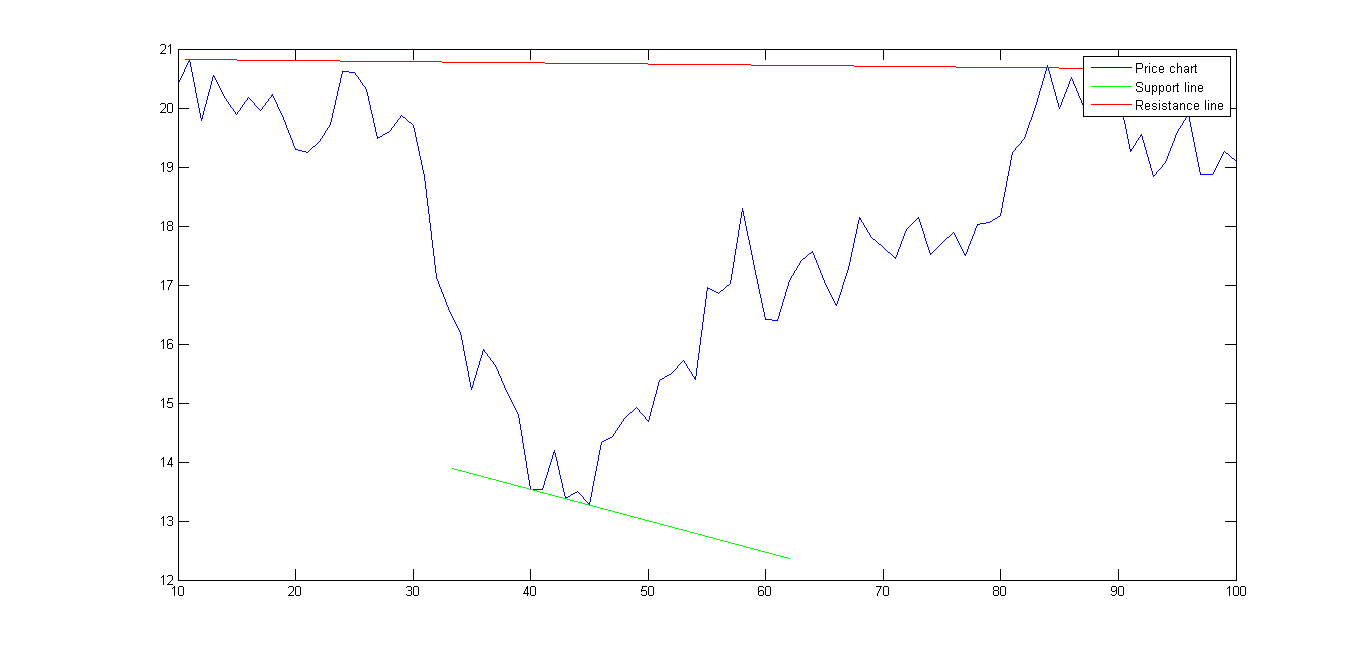
\includegraphics[width=\textwidth]{images/3.png}
    \end{center}
    \caption{Resistance and Support lines drawed by Matlab}
    \label{fig:rs}
\end{figure}  


\end{frame}

\begin{frame}
    \frametitle{Evaluation of Task 1}
It fulfills the goal of the algorithm quite well.However, it is not good enough to draw real support and resistance lines:
\begin{figure}[h]
    \begin{center}
        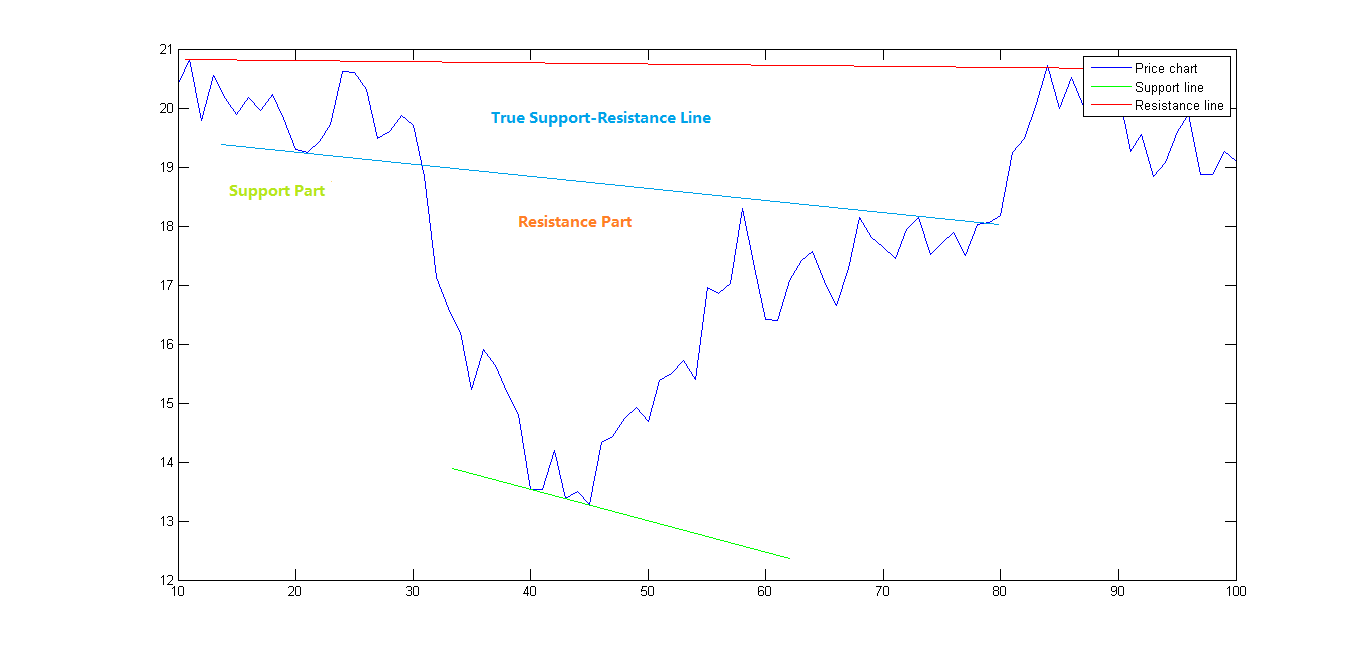
\includegraphics[width=\textwidth]{images/4.png}
    \end{center}
    \caption{Real Resistance and Support lines}
    \label{fig:rs}
\end{figure}  
\end{frame}


\begin{frame}
    \frametitle{Future Work}
\begin {itemize}
\item Improve the algorithm of Task 1, making it possible to draw multiple resistance and support lines in a give period, and the lines can be crossed by the price chart
\item Apply R to calculate covariance matrix, apply PCA analysis in Task 2\&3,
\item Optimize the stock selection.
\end{itemize}
\end{frame}
\end{document}
